\documentclass{article}

\usepackage{xeCJK,fontspec}
%\setmainfont{Times New Roman}
\setsansfont{Helvetica}
\setmonofont{Menlo Regular}

\usepackage{geometry}
\geometry{left=1cm,right=1cm,bottom=2cm,top=2cm}

\usepackage{amsmath}
\usepackage{amsfonts}
\usepackage{amssymb}
\usepackage{graphicx}
\usepackage{float}
\usepackage{indentfirst}
\usepackage{wrapfig}
\usepackage{feynmf}

\usepackage[colorlinks,linkcolor=blue]{hyperref}

\linespread{1.1}


\setCJKmainfont[BoldFont=SimHei,ItalicFont=KaiTi]{SimSun}

\renewcommand{\figurename}{\emph{图}}
\renewcommand{\tablename}{\emph{表}}

\title{\bf{在\LaTeX 中使用$\mathbf{feynmf}$宏包绘制费曼图}}

\author{\emph{清华大学\, 物理系 \, 解放}}
\date{}
\begin{document}
\maketitle
\section{引言}
在理论物理学中费曼图是一个非常实用而且常用的工具, 高能物理和凝聚态物理中都需要借助费曼图做微扰展开计算关联函数或者散射振幅. 因此对于物理学工作者常常需要向 \LaTeX 文档中插入费曼图. 但是目前互联网上并没有太完整的宏包使用方法中文文档, 因此就整理了一点采用 feynmf 包画费曼图的方法. 很惭愧, 就做了一点微小的工作, 谢谢大家.

\section{环境}
作者的使用环境为 Mac OS X 10.11.2, 采用 XeLaTeX 进行编译\footnote{采用 XeLaTeX 的原因是因为它比较方便修改字体以及支持中日韩文字, 所以写这个文档需要用, 但是多数时候并不是必须的, 直接用 LaTeX 也是可以的.}, 使用的软件就是 MacTeX 自带的 TeXShop. MacTeX 已经包含了绘制费曼图所需的宏包, 因此不需要另行下载, 直接调用即可. 对于 Windows 和 Linux 用户需要到 ctan 上下载. 下载链接: \url{http://ctan.org/pkg/feynmf}

\section{绘制}
\subsection{基本的绘制方法}
绘制费曼图, 第一步是调用 feynmf 宏包: 在导言区加入
\begin{verbatim}
\usepackage{feynmf}
\end{verbatim}
然后当我们需要插入一张费曼图时, 可以引入一个环境 fmffile 并加上一个命名\#\#\#(可以替换为合适的名称, 如 graph1, graph2...),在这个环境里面再调用 fmfgraph 环境, 就可以进行费曼图的绘制了. 写法如下:
\begin{verbatim}
\begin{fmffile}{###}
  \begin{fmfgraph}(x,y)
    ......
  \end{fmfgraph}
\end{fmffile}
\end{verbatim}
其中小括号内的数字描述的是整张费曼图的大小.

首先可以定义整张图左侧和右侧的外点, 然后通过光子线, 费米子线, 标量粒子线等等, 将外点和内点连接起来就得到一张费曼图. 定义左侧外点的指令是\verb+\fmfleft{i1,i2,...}+; 定义右侧外点的指令是\verb+\fmfright{o1,o2,...}+; 图内顶点不需要专门声明, 在连传播子的指令中出现就可以;光子线,费米子线等等传播子可以用\verb+\fmf{photon}{v1,o2}+或者类似\verb+\fmf{fermion}{i1,v1,o1}+等写法来连接不同的外点和顶点. 对于标量可以使用\verb+\fmf{plain}{i1,v1}+, \verb+\fmf{scalar}{i1,v1}+或者\verb+\fmf{dashes}{i1,v1}+等写法. \verb+plain+表示的是没有箭头的实线, 实空间中的标量场常采用这种记号; \verb+scalar+是加了箭头的虚线, 常用于动量空间中的标量场; \verb+dashes+就是没有箭头的虚线. 其他传播子的具体写法在后面会有表格总结. 

最后再介绍几个常用的参数和指令的用法:
\begin{itemize}
\item \verb+\fmf{fermion,tension=1/3}+ 表示将费米子线的"张力"调整为原来的$1/3$. 由于绘制费曼图时各条线之间的夹角是由各线上的``张力平衡''给出的, 因此有时需要调整张力使得图形更美观. 默认值为1.
\item \verb+\fmf{fermion,left=1}+ 表示将这条线画成半圆. 这在绘制圈图时非常常用. \verb+left+ 和\verb+right+分别表示像两个方向弯曲的园弧线, 参数值表示圆弧占圆周的比例, 默认值为1, 表示半圆.
\item \verb+\fmfdot{v1}+ 可以用来将顶点加粗强调.
\end{itemize}

\subsection{注意事项}
在进行绘制费曼图时有以下几点需要注意:
\begin{itemize}
\item
经过作者的测试, 在写好绘制费曼图的代码之后进行一遍编译, 会在指定位置出现"Feynman Diagram"一个短语; 经过第二遍编译之后才会出现所需要的费曼图.
\item
在写出
\begin{verbatim}
\begin{fmffile}{###}
...
\end{fmffile}
\end{verbatim}
并编译之后, .tex 文档所在的文件夹下面会一组由 \#\#\# 命名的文档, 所以说绘制多个费曼图时, 记得 \#\#\# 的命名不要重复.
\item 如果某一个费曼图的画法写错了而又完成了两次编译, 则此时需要到 .tex 文档所在的文件夹中删除与这幅图相关的那些文件的内容. 修改费曼图的画法之后再进行编译, 可以将其修正.
\end{itemize}

\section{样例}
\subsection{作为浮动体插入费曼图}
在这一段我们以$e^{-}\gamma\rightarrow e^{-}\gamma$ 树图阶康普顿散射为例, 示范如何绘制作为图片插入费曼图.\\
示范代码:
\begin{verbatim}
\begin{figure}[!htp]
\centering
\begin{fmffile}{graph1}
  \begin{fmfgraph}(110,60)
    \fmfleft{i1,i2}
    \fmfright{o1,o2}
    \fmf{fermion}{i2,v2,v1,o1}
    \fmf{photon}{i1,v1}
    \fmf{photon}{v2,o2}
  \end{fmfgraph}
\end{fmffile}
\caption{A scattering process (u-channel) of Campton experiment}
\end{figure}
\end{verbatim}

其输出效果如下图所示:
\begin{figure}[!htp]
\centering
\begin{fmffile}{graph1}
  \begin{fmfgraph}(110,60)
    \fmfleft{i1,i2}
    \fmfright{o1,o2}
    \fmf{fermion}{i2,v2,v1,o1}
    \fmf{photon}{i1,v1}
    \fmf{photon}{v2,o2}
  \end{fmfgraph}
\end{fmffile}
\caption{A scattering process (u-channel) of Campton experiment}
\end{figure}\\
此时我们就得到了第一张费曼图. 注意在我们的代码中, 左侧外点\verb+i1+ 连接的是光子, 而左侧外点\verb+i2+连接的是电子. 从图中可以看出, 外点是按从下到上排列的. 右侧外点的情况也是一样的. 在后面的例子中我们也会发现相同的现象.

\subsection{圈图}
圈图的画法有一些需要注意的地方, 因此单独拿出一节来讨论. 下面还是以一些例子来解释圈图的画法.
\subsubsection{四顶点正负电子湮灭项}
最简单的圈图并不需要画弯曲的传播子, 按照树图的画法去写命令就可以了. 例如正负电子对湮灭的四顶点修正项, 其写法如下:
\begin{verbatim}
\begin{fmffile}{graph2}
  \begin{fmfgraph}(110,60)
    \fmfleft{i1,i2}
    \fmfright{o1,o2}
    \fmf{fermion}{i1,v1,v2,v3,v4,i2}
    \fmf{photon}{v1,v4}
    \fmf{photon}{v2,o1}
    \fmf{photon}{v3,o2}
    \fmfdot{v1,v2,v3,v4}
  \end{fmfgraph}
\end{fmffile}
\end{verbatim}
注意到\verb+\fmfdot{}+指令: 此处我们已经将所有的顶点加粗. 输出效果如下图所示:
\begin{figure}[!htp]
\centering
\begin{fmffile}{graph2}
  \begin{fmfgraph}(110,60)
    \fmfleft{i1,i2}
    \fmfright{o1,o2}
    \fmf{fermion}{i1,v1,v2,v3,v4,i2}
    \fmf{photon}{v1,v4}
    \fmf{photon}{v2,o1}
    \fmf{photon}{v3,o2}
    \fmfdot{v1,v2,v3,v4}
  \end{fmfgraph}
\end{fmffile}
\caption{\emph{正负电子对湮灭的高阶修正}}
\end{figure}\\
很明显, \emph{图} 2 相对于 \emph{图} 1 最显著的区别就是顶点全部都被描黑了.

\subsubsection{标量场自作用}
首先来看一下$\phi^4$自作用标量场的真空极化项. 按照最简单的想法, 最低阶的一顶点修正写法如下所示:
\begin{verbatim}
\begin{fmffile}{graph3}
  \begin{fmfgraph}(110,60)
   \fmfleft{i1}
   \fmfright{o1}
   \fmf{plain}{i1,v1}
   \fmf{plain}{v1,o1}
   \fmf{plain}{v1,v1}
 \end{fmfgraph}
\end{fmffile}
\end{verbatim}
上述代码的实线效果图:
\begin{figure}[!htp]
\centering
\begin{fmffile}{graph3}
  \begin{fmfgraph}(110,60)
   \fmfleft{i1}
   \fmfright{o1}
   \fmf{plain}{i1,v1}
   \fmf{plain}{v1,o1}
   \fmf{plain}{v1,v1}
 \end{fmfgraph}
\end{fmffile}
\caption{\emph{$\phi^4$标量场的真空极化}}
\end{figure}\\
这里可以看出, 对于两端连在一起的传播子, 并不需要特别的设置就可以了. 如果把上面例子中的\verb+plain+换成\verb+scalar+, 就是动量\newpage 空间中的标量场自作用图了:
\begin{figure}[!htp]
\centering
\begin{fmffile}{auxgraph1}
  \begin{fmfgraph}(110,60)
   \fmfleft{i1}
   \fmfright{o1}
   \fmf{scalar}{i1,v1}
   \fmf{scalar}{v1,o1}
   \fmf{scalar}{v1,v1}
 \end{fmfgraph}
\end{fmffile}
\end{figure}\\
下面再来看一个例子: $\phi^6$ 标量场的真空极化一顶点项, 其命令应该按照下述写法:
\begin{verbatim}
\begin{fmffile}{graph4}
  \begin{fmfgraph}(110,60)
   \fmfleft{i1}
   \fmfright{o1}
   \fmf{plain}{i1,v1}
   \fmf{plain}{v1,o1}
   \fmf{plain}{v1,v1}
   \fmf{plain,left}{v1,v1}
 \end{fmfgraph}
\end{fmffile}
\end{verbatim}
其中的一个圈需要通过 \verb+left+指令进行转向, 把它翻到下方来画, 否则两个圈重叠起来, 就不是我们所需要的那个图了. 效果如下:
\begin{figure}[!htp]
\centering
\begin{fmffile}{graph4}
  \begin{fmfgraph}(110,60)
   \fmfleft{i1}
   \fmfright{o1}
   \fmf{plain}{i1,v1}
   \fmf{plain}{v1,o1}
   \fmf{plain}{v1,v1}
   \fmf{plain,left}{v1,v1}
 \end{fmfgraph}
\end{fmffile}
\caption{\emph{$\phi^6$场的真空极化}}
\end{figure}

\subsubsection{光子真空极化}
两顶点的圈图比较特殊, 需要把连线画成弯曲的, 因此直接套用树图的画法是不行的. 首先看下面一段 TeX 代码:
\begin{verbatim}
    \fmfleft{i1}
    \fmfright{o1}
    \fmf{photon}{i1,v1}
    \fmf{fermion}{v1,v2,v1}
    \fmf{photon}{v2,o1}
\end{verbatim}
但是编译输出后的结果如下所示:
\begin{figure}[!htp]
\centering
\begin{fmffile}{auxgraph2}
  \begin{fmfgraph}(110,60)
    \fmfleft{i1}
    \fmfright{o1}
    \fmf{photon}{i1,v1}
    \fmf{fermion}{v1,v2,v1}
    \fmf{photon}{v2,o1}
  \end{fmfgraph}
\end{fmffile}
\end{figure}\\
可见, 通过上述写法得到的费曼图是不行的, 两条直的费米子线重叠在一起了. 因此这时需要使用 \verb+left+或\verb+right+指令. 最简单的情况如下:
\begin{verbatim}
\begin{fmffile}{graph5}
  \begin{fmfgraph}(110,60)
   \fmfleft{i1}
   \fmfright{o1}
   \fmf{photon}{i1,v1}
   \fmf{fermion,left}{v1,v2,v1}
   \fmf{photon}{v2,o1}
 \end{fmfgraph}
\end{fmffile}
\end{verbatim}
这时参数 \verb+left+ 为其默认值 1. 输出效果如下图:
\begin{figure}[!htp]
\centering
\begin{fmffile}{graph5}
  \begin{fmfgraph}(110,60)
   \fmfleft{i1}
   \fmfright{o1}
   \fmf{photon}{i1,v1}
   \fmf{fermion,left}{v1,v2,v1}
   \fmf{photon}{v2,o1}
 \end{fmfgraph}
\end{fmffile}
\caption{\emph{光子真空极化}}
\end{figure}
\\如果调节上述指令中的\verb+\left+参数值, 费曼图会发生如下变化:
\begin{figure}[!htp]
\centering
\begin{fmffile}{auxgraph3}
  \begin{fmfgraph}(110,60)
   \fmfleft{i1}
   \fmfright{o1}
   \fmf{photon}{i1,v1}
   \fmf{fermion,left=0.5}{v1,v2,v1}
   \fmf{photon}{v2,o1}
 \end{fmfgraph}
 \begin{fmfgraph}(110,60)
   \fmfleft{i1}
   \fmfright{o1}
   \fmf{photon}{i1,v1}
   \fmf{fermion,left=1.5}{v1,v2,v1}
   \fmf{photon}{v2,o1}
 \end{fmfgraph}
\end{fmffile}
\end{figure}\\
左侧费曼图的参数\verb+left=0.5+, 右侧费曼图的参数\verb+left=1.5+.

\subsubsection{电子自能}
电子自能图一般不会把电子线画成弯的, 因为这样会使得费曼图很不美观. 我们一般将其分成三段来画:
\begin{verbatim}
\begin{fmffile}{graph6}
  \begin{fmfgraph}(110,60)
   \fmfleft{i1}
   \fmfright{o1}
   \fmf{plain}{i1,v1}
   \fmf{fermion}{v1,v2}
   \fmf{photon,left}{v1,v2}
   \fmf{plain}{v2,o1}
 \end{fmfgraph}
\end{fmffile}
\end{verbatim}
效果如下
\begin{figure}[!htp]
\centering
\begin{fmffile}{graph6}
  \begin{fmfgraph}(110,60)
   \fmfleft{i1}
   \fmfright{o1}
   \fmf{plain}{i1,v1}
   \fmf{fermion}{v1,v2}
   \fmf{photon,left}{v1,v2}
   \fmf{plain}{v2,o1}
 \end{fmfgraph}
\end{fmffile}
\caption{\emph{电子的自能图}}
\end{figure}\\
这时候由于变成了三根线, 需要考虑到\verb+tension+参数的影响了. QED 中的一个顶点会连接一进一出的两个电子线和一个光子线. 如果某一条电子线换成自能图, 那该怎么写? 顺着上面例子的思路, 似乎可以写出如下的指令:
\begin{verbatim}
    \fmfleft{i1,i2}
    \fmfright{o1}
    \fmf{fermion}{i1,v1}
    \fmf{plain}{v1,v2}
    \fmf{fermion}{v2,v3}
    \fmf{plain}{v3,i2}
    \fmf{photon,right}{v2,v3}
    \fmf{photon}{v1,o1}
\end{verbatim}
然而输出的效果并不好, 如下图所示, 上下两条电子线已经明显偏斜了, 不美观.
\begin{figure}[!htp]
\centering
\begin{fmffile}{auxgraph4}
  \begin{fmfgraph}(220,120)
    \fmfleft{i1,i2}
    \fmfright{o1}
    \fmf{fermion}{i1,v1}
    \fmf{plain}{v1,v2}
    \fmf{fermion}{v2,v3}
    \fmf{plain}{v3,i2}
    \fmf{photon,right}{v2,v3}
    \fmf{photon}{v1,o1}
 \end{fmfgraph}
\end{fmffile}
\end{figure}\\
此时我们可以将下面那条电子线的张力减小到之前的三分之一, 即令\verb+tension=1/3+, 然后再把虚光子的张力调整为零, 即令\verb+tension=0+, 如下所示:
\begin{verbatim}
\begin{fmffile}{graph7}
  \begin{fmfgraph}(180,100)
    \fmfleft{i1,i2}
    \fmfright{o1}
    \fmf{fermion,tension=1/3}{i1,v1}
    \fmf{plain}{v1,v2}
    \fmf{fermion}{v2,v3}
    \fmf{plain}{v3,i2}
    \fmf{photon,right,tension=0}{v2,v3}
    \fmf{photon}{v1,o1}
 \end{fmfgraph}
\end{fmffile}
\end{verbatim}
这时的效果如下:
\begin{figure}[!htp]
\centering
\begin{fmffile}{graph7}
  \begin{fmfgraph}(180,100)
    \fmfleft{i1,i2}
    \fmfright{o1}
    \fmf{fermion,tension=1/3}{i1,v1}
    \fmf{plain}{v1,v2}
    \fmf{fermion}{v2,v3}
    \fmf{plain}{v3,i2}
    \fmf{photon,right,tension=0}{v2,v3}
    \fmf{photon}{v1,o1}
 \end{fmfgraph}
\end{fmffile}
\caption{\emph{调整之后的费曼图}}
\end{figure}


\subsection{作为表达式的一部分插入费曼图}
费曼图表示一个积分, 所以我们有时不需要把它们当成浮动体, 而是公式的一部分插入到文档中. 下面两个式子分别是光子自能和卢瑟福散射实验($e^-p^+\rightarrow e^-p^+$)的费曼图和相应的表达式, 指令如下:
\begin{verbatim}
\begin{fmffile}{equation}
  \begin{eqnarray}
    \parbox{30mm}{\begin{fmfgraph}(80,50) \fmfleft{i1} \fmfright{o1} \fmf{photon}{i1,o1} 
    \end{fmfgraph}}\quad + \quad\parbox{30mm}{\begin{fmfgraph}(80,50) \fmfleft{i1} 
    \fmfright{o1}\fmf{photon}{i1,v1} \fmf{fermion,left}{v1,v2,v1} \fmf{photon}{v2,o1} 
    \end{fmfgraph}} \quad &\simeq& \frac{-i g_{\mu\nu}}{p^2+ \Pi(p^2) +i \epsilon}\\
    (-ie)^2\bar{u}(p_3)\gamma^{\mu}u(p_1)
    \frac{-i g_{\mu\nu}}{(p_1-p_3)^2}\bar{u}(p_4)\gamma^\nu u(p_2) &=& \parbox{20mm}{
    \begin{fmfgraph}(40,60) \fmfleft{i1,i2} \fmfright{o1,o2} \fmf{fermion}{i1,v1,o1} 
    \fmf{fermion}{i2,v2,o2} \fmf{photon}{v1,v2} \end{fmfgraph}
    }
  \end{eqnarray}
\end{fmffile}
\end{verbatim}
输出效果如下所示:
\begin{fmffile}{equation}
  \begin{eqnarray}
    \parbox{30mm}{\begin{fmfgraph}(80,50) \fmfleft{i1} \fmfright{o1} \fmf{photon}{i1,o1} 
    \end{fmfgraph}}\quad + \quad\parbox{30mm}{\begin{fmfgraph}(80,50) \fmfleft{i1} \fmfright{o1}
    \fmf{photon}{i1,v1} \fmf{fermion,left}{v1,v2,v1} \fmf{photon}{v2,o1} 
    \end{fmfgraph}} \quad &\simeq& \frac{-i g_{\mu\nu}}{p^2+ \Pi(p^2) +i \epsilon}\\
    (-ie)^2\bar{u}(p_3)\gamma^{\mu}u(p_1)
    \frac{-i g_{\mu\nu}}{(p_1-p_3)^2}\bar{u}(p_4)\gamma^\nu u(p_2) &=& \parbox{20mm}{
    \begin{fmfgraph}(40,60) \fmfleft{i1,i2} \fmfright{o1,o2} \fmf{fermion}{i1,v1,o1} 
    \fmf{fermion}{i2,v2,o2} \fmf{photon}{v1,v2} \end{fmfgraph}}
  \end{eqnarray}
\end{fmffile}
最常用的几类费曼图的画法大概就是这样.
\newpage
\section{附录: 关于不同的传播子的指令}
作者偷懒, 截图示意了:
\begin{figure}[!htp]
\centering
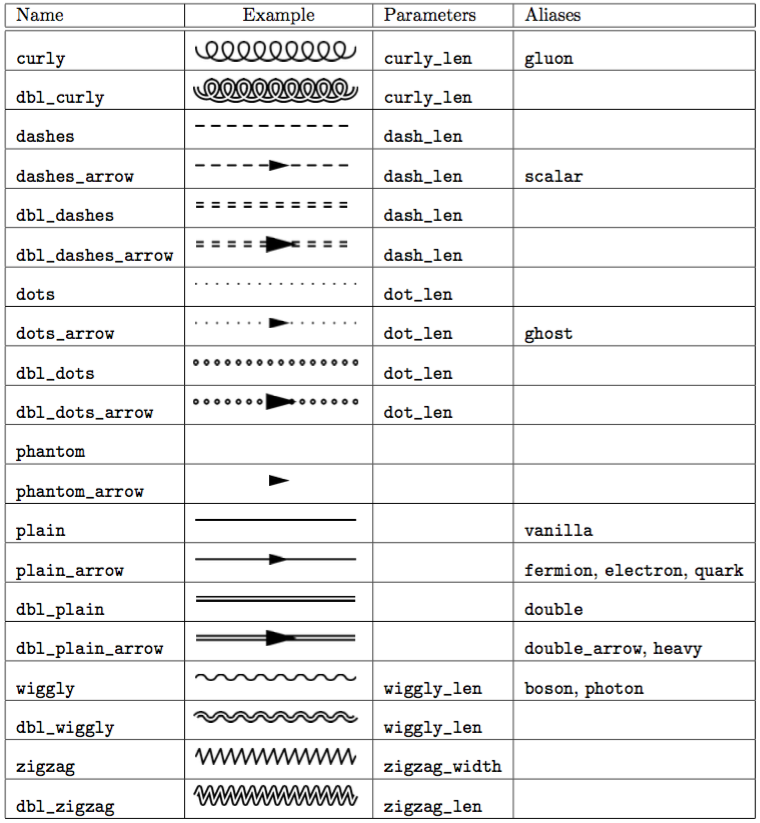
\includegraphics[width=15cm]{propagator.png}
\caption{\emph{各种各样的传播子}}
\end{figure}

关于费曼图的绘制还有很多需要注意的地方, 比如说为传播子和顶点添加标记, 其他形状的(例如多边形)顶点等等.更详细的说明应该去参考\TeX 文档中关于 fenmf 宏包的部分.
\end{document}








